\section{Example}
In this section the motivating example of the work in explained. First a immutable class is presented, a case is shown when it is safe to transform the class to an immutable class. Following the positive example, a case is presented which explains when it is not possible to transform an immutable class to mutable. The point of the analysis is to recognize the cases when an object cannot be transformed to mutable due to the nature of its usage by the caller of the object.
%The Immutable class

\begin{figure}[H]
	\caption{Immutable Object} \label{fig:immutable_object}
	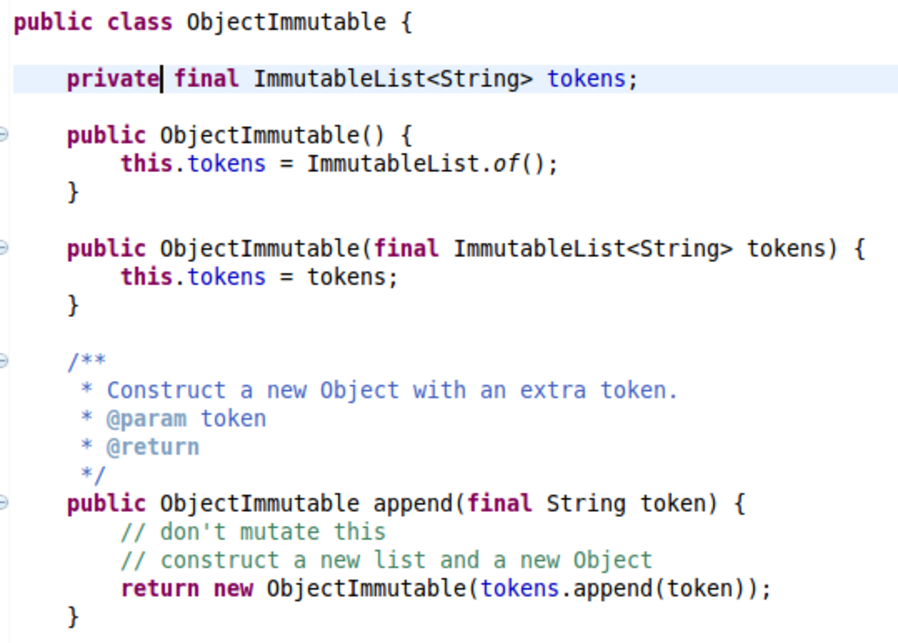
\includegraphics[width=0.5\textwidth]{img/immutable_object}
\end{figure}

\begin{figure}[H]
	\caption{Client without object escaping} \label{fig:clientNoEscape}
	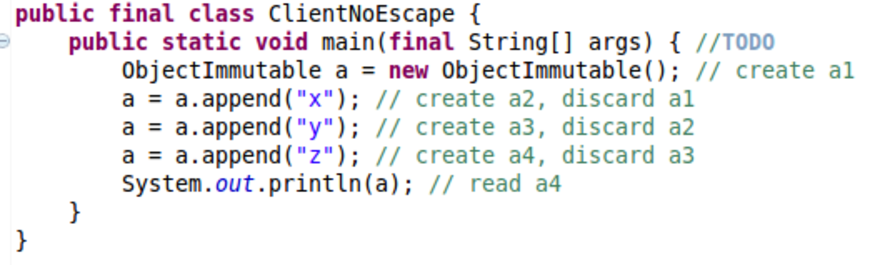
\includegraphics[width=0.5\textwidth]{img/client_noescape}
\end{figure}

In this example object shown in figure \ref{fig:immutable_object} it is evident that the object is immutable by the fact that the \texttt{token} attribute is \textit{final} and that the mutator method, \texttt{append\(\)} returns an instance of the mutated object rather than mutating the subject instance and returning \texttt{void}. Now let's look at figure \ref{fig:clientNoEscape} which shows the instance of an client object calling the immutable object. In this method all that is happening is that the client is appending to the initially created instance and finally it prints the most recent instance to the console. In this case, since the initialized immutable object is not assigned to other globally accessible varible such as a \texttt{static} variable, or that it is not being passed as a parameter to another method, it is evident that within this caller, the object is not ``escaping''. The conditions for escape analysis that are used in this project are discussed later on in section \ref{sec:escape}.
Therefore if the this is the only client calling the the immutable object then it would be safe to transform the immutable object to an mutable object, because a reference of the object is not assigned to the heap before the end of execution of the method.

\begin{figure}[H]
	\caption{Transformed Mutable Object} \label{fig:mutableobj}
	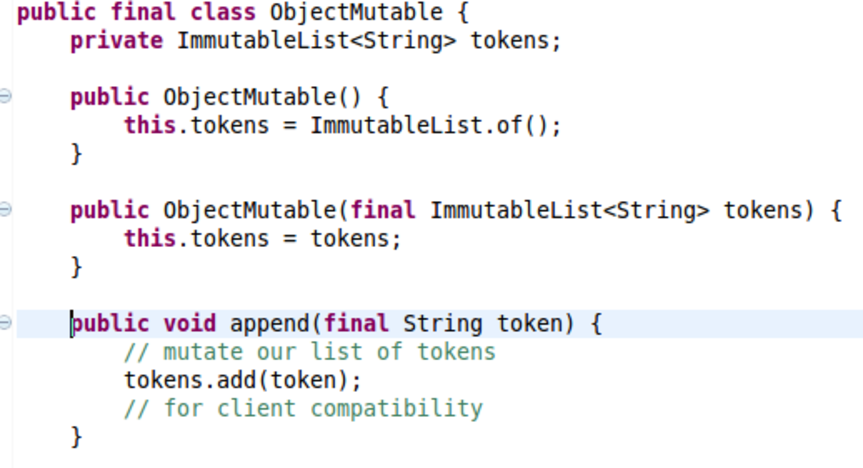
\includegraphics[width=0.5\textwidth]{img/mutable_object}
\end{figure}

\begin{figure}[H]
	\caption{Transformed Client Object} \label{fig:transformedclient}
	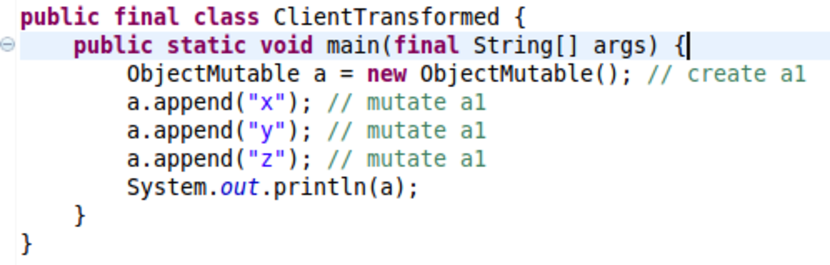
\includegraphics[width=0.5\textwidth]{img/client_transformed}
\end{figure}

A possible transformation of the immutable object can be viewed in figure \ref{fig:mutableobj}. In figure \ref{fig:mutableobj} it is evident that that only difference the immutable object and this are three transformations:
\begin{itemize}
\item The local variable has been changed from \texttt{private final} to just \texttt{private}.
\item The mutator method \texttt{append} has been changed to return a \texttt{void} type.
\item The mutator method directly appends to the \texttt{ImmutableList}.
\end{itemize}

Because of the change in the object implementation. All the calling sites of the object also needs to be refactored in order to make this change effective. In figure \ref{fig:transformedclient} the transformed client is shown. The changes that happen to the client are the program points where the client calls the mutator method of the transformed mutable object.

\begin{figure}[H]
	\caption{Client with Escaping Object} \label{fig:client_escape}
	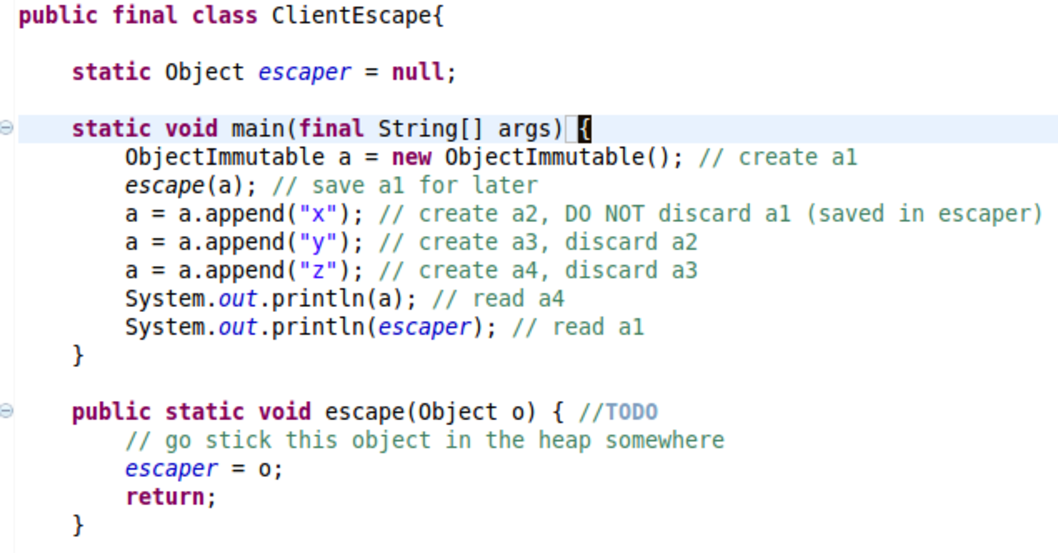
\includegraphics[width=0.5\textwidth]{img/client_escape}
\end{figure}

Figure \ref{fig:client_escape} presents an example of a client where an object is escaping the stacking and is creating a pointer to the heap. The points to note here is that at the second line of the metho, the instantiated Immutable object is being passed as a parameter to a method. Inside the \texttt{escape()} method, the immutable object is assigned to a static global variable. Since global variable can be accessed multiple methods, this causes the immutable object to have a reference to the heap which causes it to be globally accessible. This is a case when an object is said to have ``escaped''. Turning attention to the main method again, it can be noticed that at the end of the method, the method is using the assigned static global variable \texttt{escaper} which stores a reference in the heap for the first instance of the local variable \texttt{a}. Now since the local object was immutable in nature, the heap reference stores the original instance, and when the global variable is referenced at a subsequent program point it successfully returns the original instance of the object. However, if the local object was mutable instead, it would lose its original instance through the mutator methods between the program point where  the object is escaping and when the escaped object is being referenced at a later program point. So an erroneous value for the local object would be returned. The objective of this analysis is to detect this use cases through escape analysis and detect which objects in a method can be transformed to mutable.
%Its Safe to mutate client
%What it is safe to convert t
%The Case where it cannot be transformed
%Explain object escaping